%================================================================================
%\appsection[CBTI and Quadrature]{quad}{Relationship between CBTI and Quadrature Integration}
%================================================================================



\section{Ligands}
\begin{center}
%\scriptsize
\resizebox{\columnwidth}{!}{%
\begin{tabular}{l | l | l}
ligand & IUPAC name & canonical SMILES (Daylight)\\
\hline
\_O6T & 1,2-Dimethoxybenzene & COc1ccccc1OC \\
\_O70 & (2R,5R)-2-methyl-5-prop-1-en-2-ylcyclohexan-1-one & CC(=C)[C@@H]1CC[C@H](C(=O)C1)C\\
\_O71 & (1S,5R)-2-methyl-5-prop-1-en-2-ylcyclohex-2-en-1-ol & CC(=C)[C@@H]1CC=C([C@H](C1)O)C\\ 
\_P8I & Cyclopentanone & O=C1CCCC1\\
6J29 & 1-amino-4-hydroxyanthracene-9,10-dione & Oc1ccc(c2c1C(=O)c1ccccc1C2=O)N\\
6KET & 3-Methoxyphenol & COc1cccc(c1)O\\
8018 & - & Cl[C@@H]1C[C@H]2[C@@H]([C@H]1Cl)[C@]1(C([C@]2(Cl)C(=C1Cl)Cl)(Cl)Cl)Cl\\
E1VB & - & F[C@H](C(F)F)Oc1ccccc1\\
F313 & 4-Methoxyaniline & COc1ccc(cc1)N\\
G078 & 1,4-Dimethylnaphthalene & Cc1ccc(c2c1cccc2)C\\
G277 & cyclohexa-2,5-diene-1,4-dione & O=C1C=CC(=O)C=C1\\
M030 & 1,3,5-Trimethylbenzene & Cc1cc(C)cc(c1)C\\
M097 & 2-Chloroaniline & Nc1ccccc1Cl\\
M218 & N-Methylaniline & CNc1ccccc1 \\
S002 & - & BrCc1ccccc1\\
TVVS & - & O=CC1=CC=[N]=CC1 \\
\end{tabular}
}
\end{center}

\section{Restraint Placement}
\begin{figure}
    \centering
    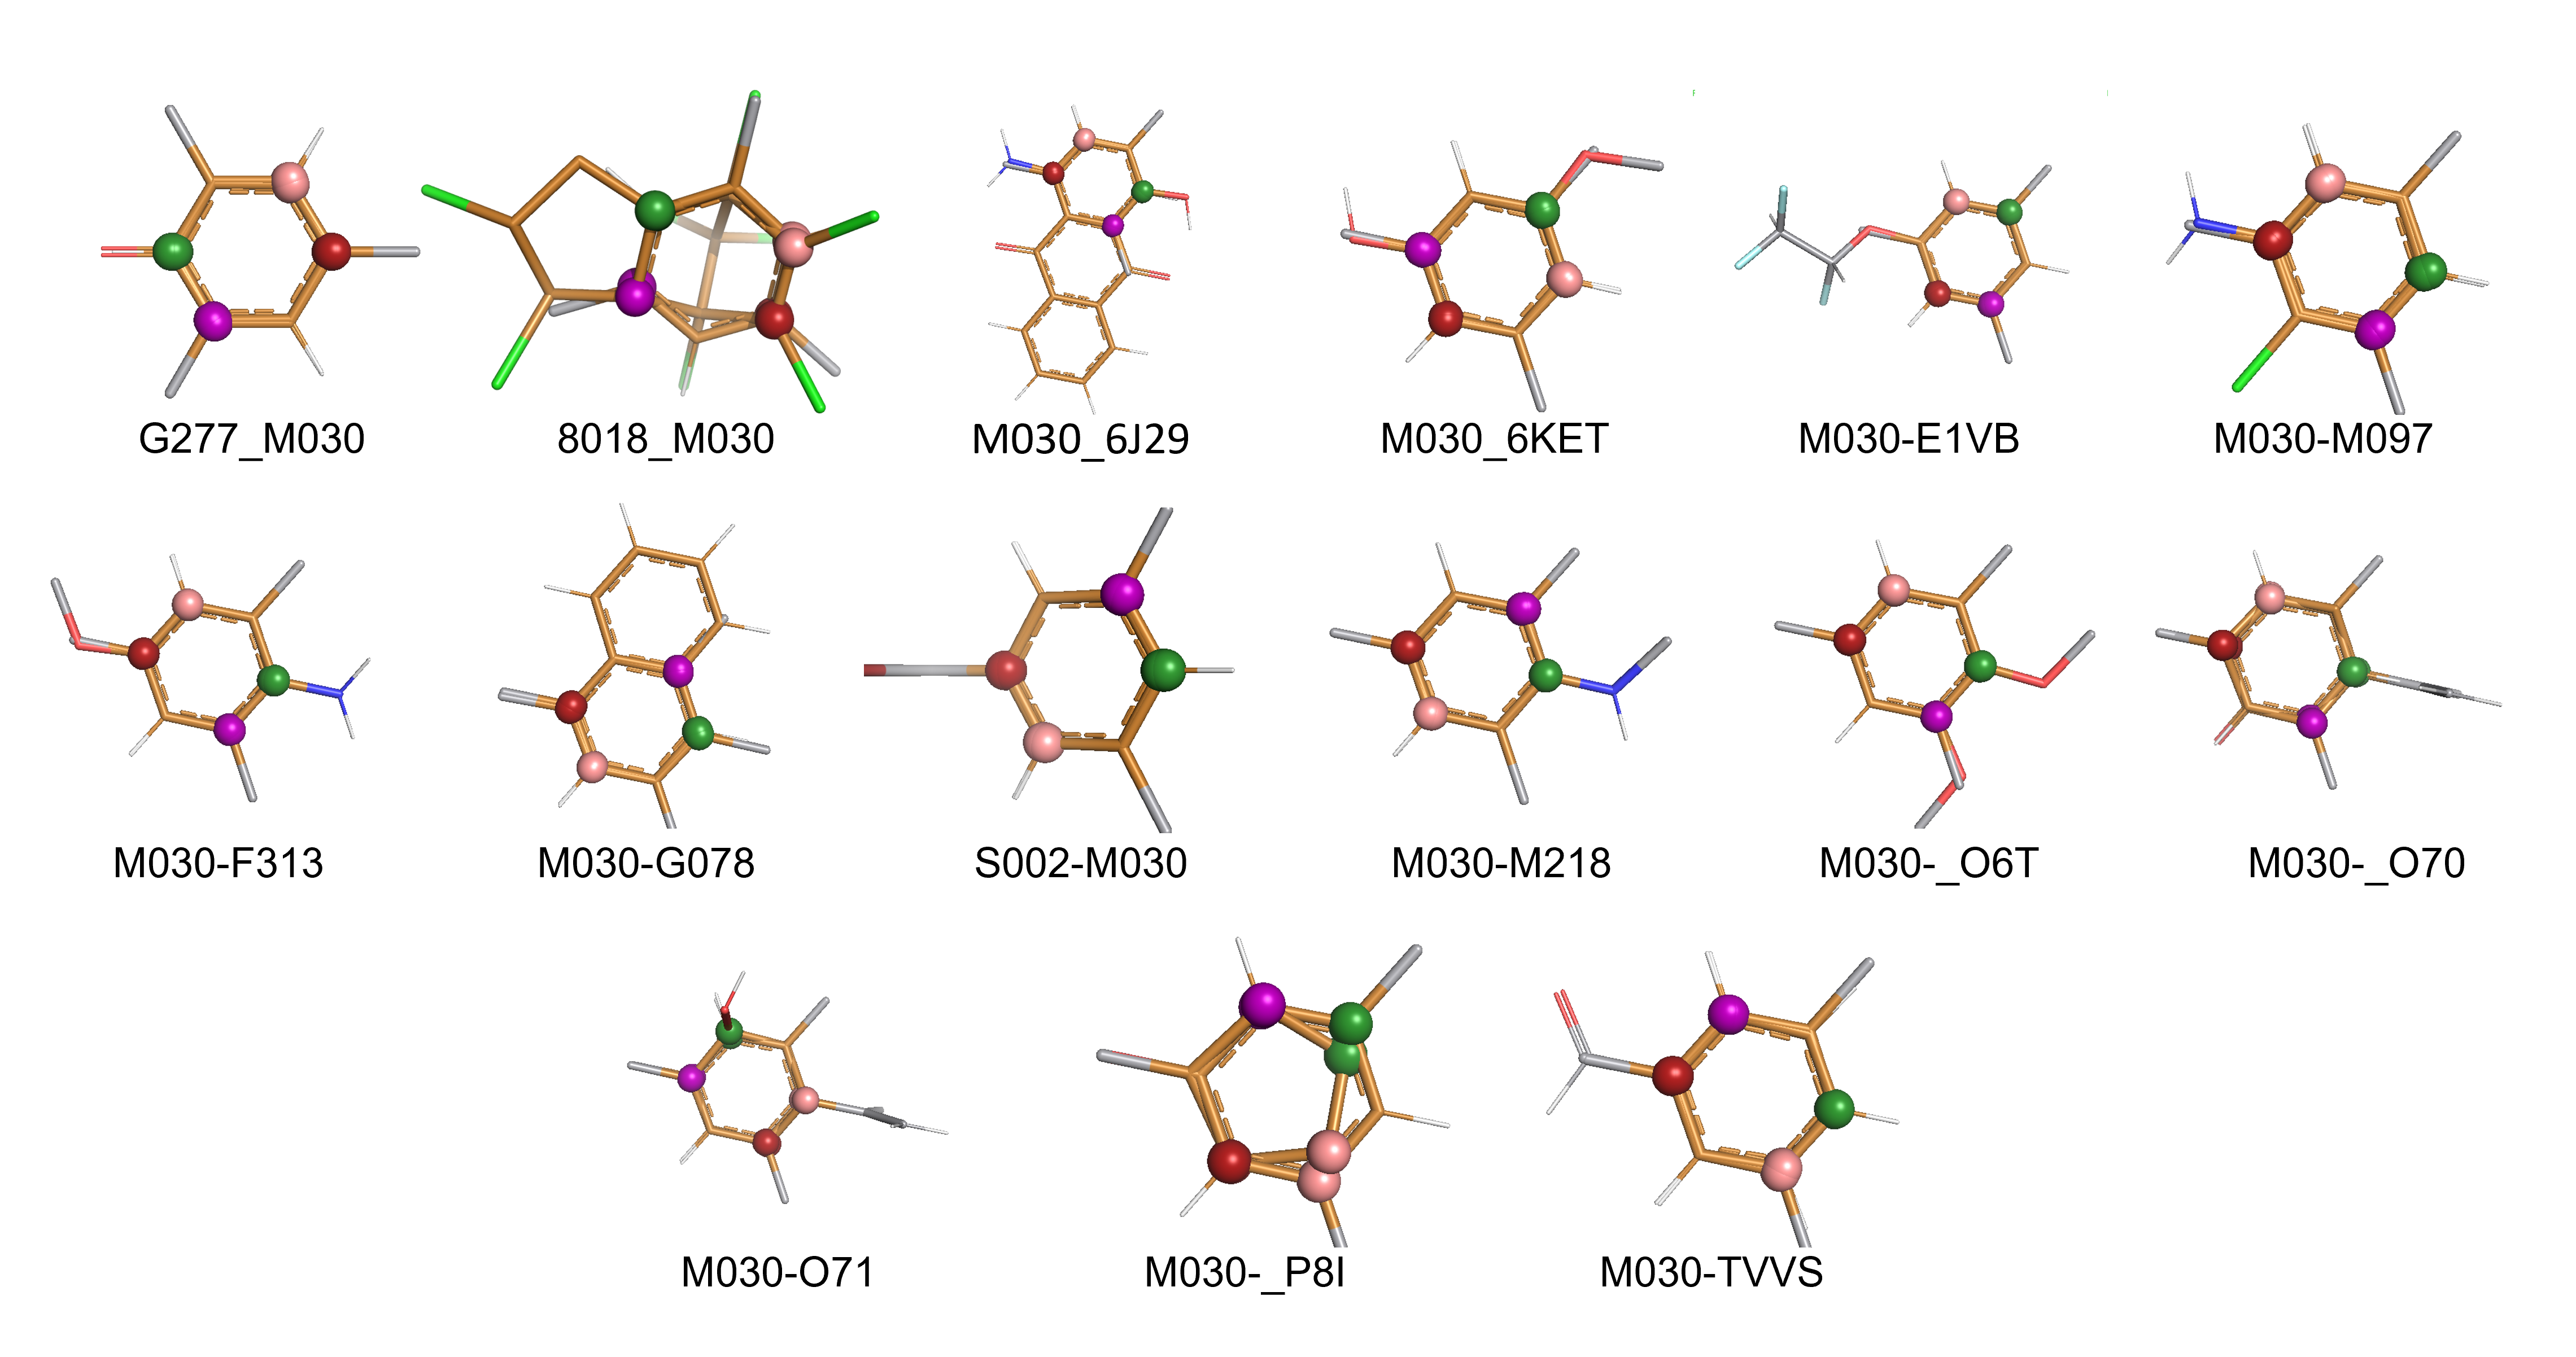
\includegraphics[width=\textwidth]{fig/results/pairwise/restraintPlacement/Restraints_PairwiseTI_M030Graph.png}
    \caption{Placement of the restraints for the pairwise TI- M030 system}
    \label{SIfig: Pairwise_TI_M030_Graph}
\end{figure}

\begin{figure}
    \centering
    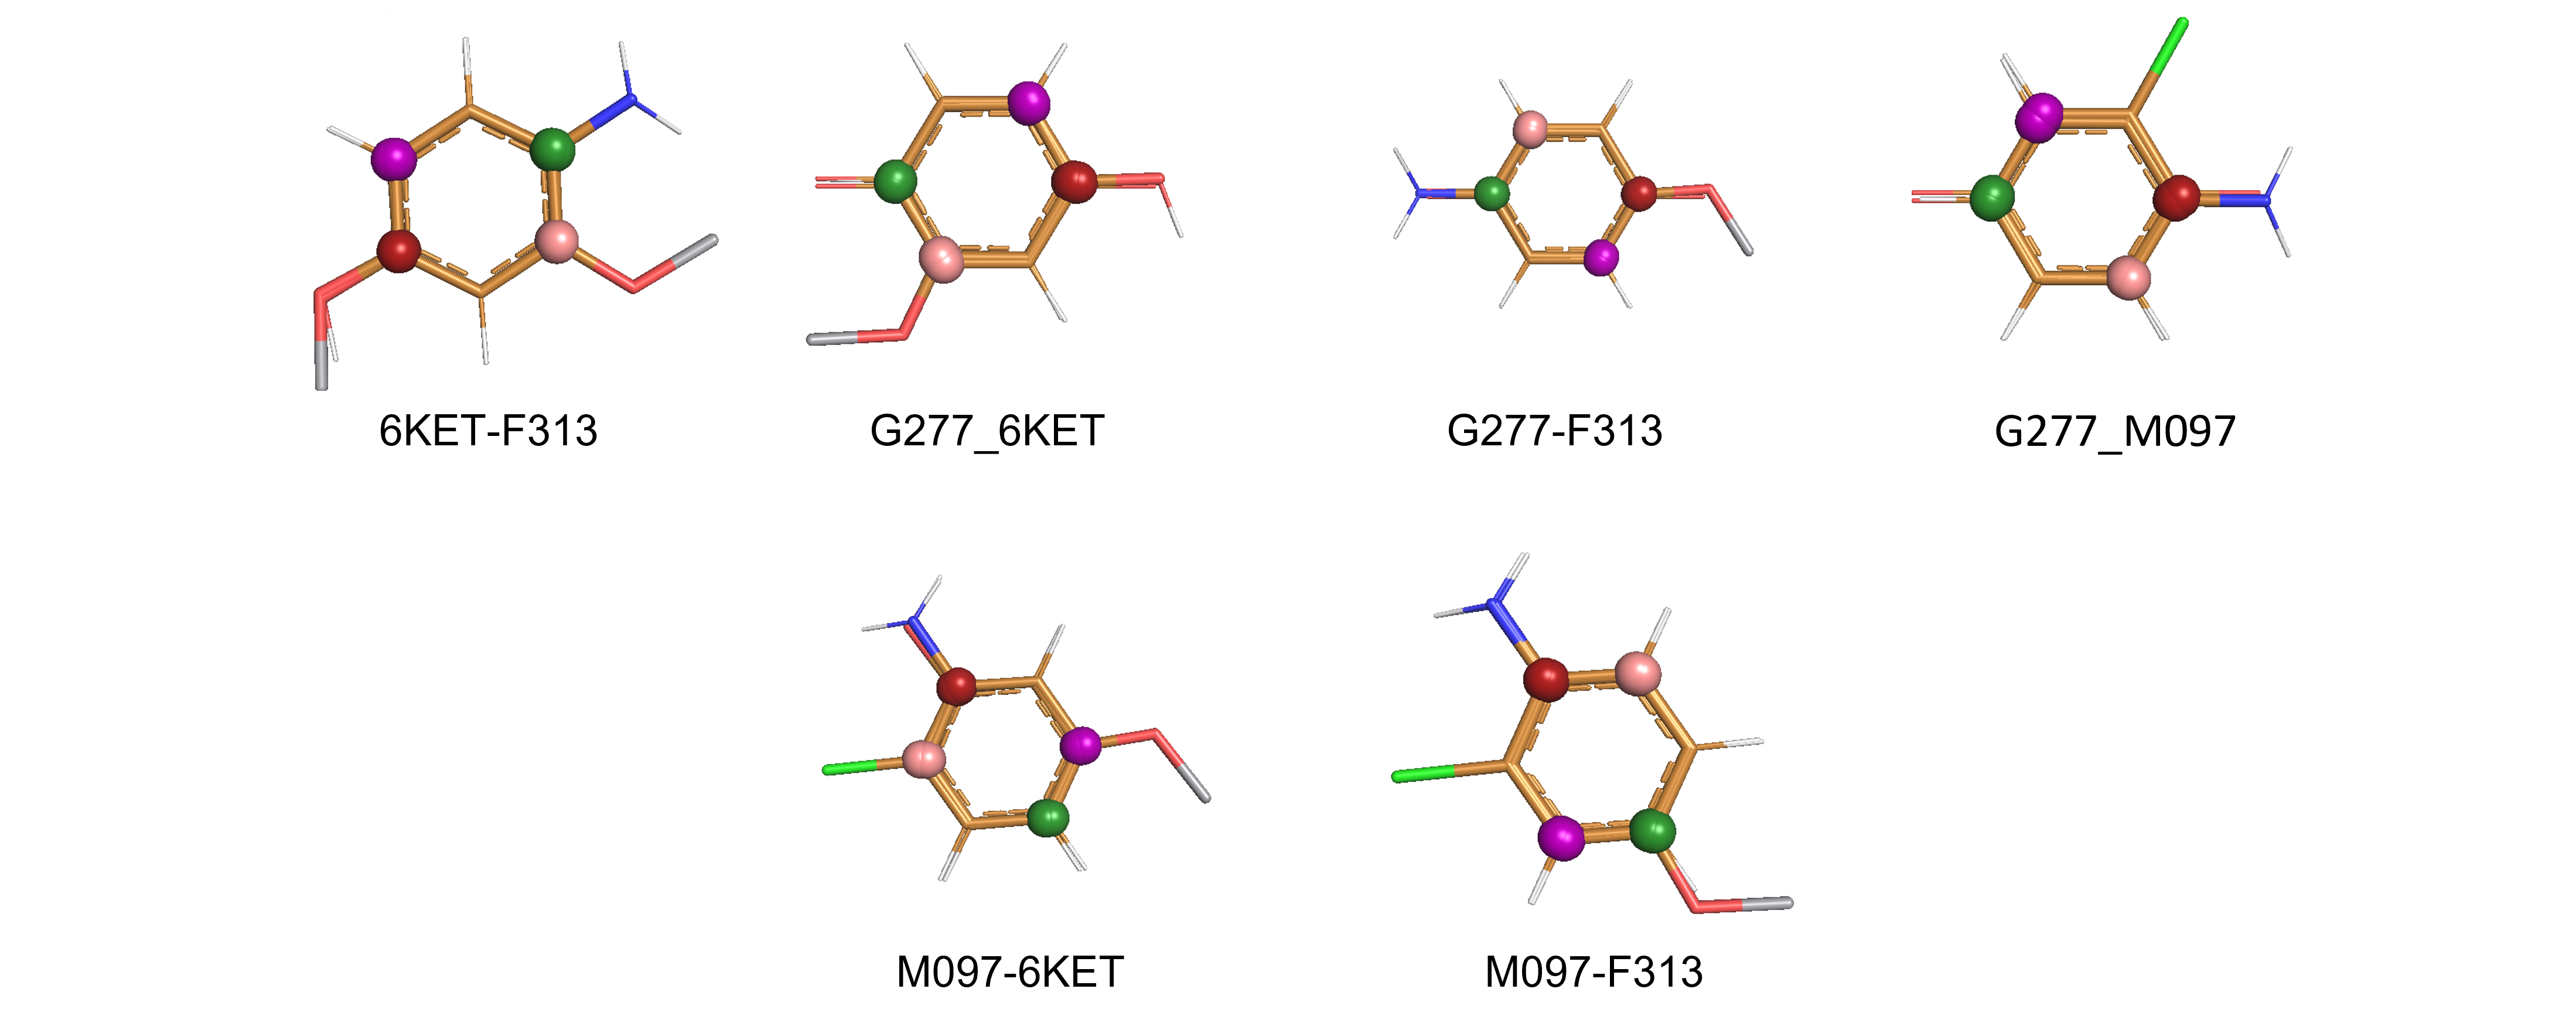
\includegraphics[width=\textwidth]{fig/results/pairwise/restraintPlacement/Restraints_PairwiseTI_reedsaddition.png}
    \caption{Placement of the restraints for the TI calculation for the full graph comparison to multistate set A}
    \label{SIfig:Pairwise_TI_AddRE-EDS_Graph}
\end{figure}

\clearpage

\section{Relative Hydration Free Energy Calculations}
\subsection{Pairwise TI}

\begin{table}[H]
\caption{Pairwise relative hydration free energies with one base molecule. Experimental data and the ABFE calculations by ATB are taken from the ATB database.\cite{Martin2018} The RAFE was calculated from the experimental and the ABFE ATB  data. The RAFE results of the TI approach use the introduced restraint approach. The uncertainty was calculated via Gaussian error propagation of the provided errors. The experimental uncertainty for the pair G277-M030 could not be provided, as the experimental uncertainty of G277 is not provided in the ATB database. The RMSE and its uncertainty were estimated with a 100 fold bootstrap approach.}
\begin{center}
%\resizebox{\columnwidth}{!}{%
\footnotesize
\begin{tabular}{ c c |c |c|c|}
  \multicolumn{2}{c|}{Ligands} & \multicolumn{1}{c|}{Experiment} &\multicolumn{1}{c|}{ATB}&\multicolumn{1}{c|}{TI}\\ 
    $i$ & $j$ & [kJ~mol$^{-1}$] & [kJ~mol$^{-1}$] & [kJ~mol$^{-1}$]  \\
  \hline
        \_O6T &  M030 &  $18.5 ~\pm~ 1.3$  &  $26.2 ~\pm~ 0.8$ &  $  17.5 ~\pm~ 0.7$\\
        \_O70 &  M030 &  $11.9 ~\pm~ 1.3$  &  $14.4 ~\pm~ 0.7$ &  $  8.6 ~\pm~ 0.6 $\\
        \_O71 &  M030 &  $14.8 ~\pm~ 1.5$  &  $22.4 ~\pm~ 0.7$ &  $ 15.2 ~\pm~ 0.9 $\\
        \_P8I &  M030 &  $15.9 ~\pm~ 1.8$  &  $15.3 ~\pm~ 0.6$ &  $  9.4 ~\pm~ 0.4 $\\
        6J29 &  M030 &   $36.1 ~\pm~ 1.4$  &  $48.2 ~\pm~ 0.4$ &  $ 46.9 ~\pm~ 0.8 $\\
        6KET &  M030 &   $28.1 ~\pm~ 1.8$  &  $36.1 ~\pm~ 0.6$ & $  30.5 ~\pm~ 0.5 $\\
        8018 &  M030 &   $10.6 ~\pm~ 1.3$  &  $22.8 ~\pm~ 0.5$ &  $  9.5 ~\pm~ 0.9 $\\
        E1VB &  M030 &   $ 1.6 ~\pm~ 1.8$  &  $ 5.2 ~\pm~ 0.7$ &  $ 3.0 ~\pm~ 1.2 $\\
        F313 &  M030 &   $27.5 ~\pm~ 1.8$  &  $30.2 ~\pm~ 0.6$ &  $ 25.7 ~\pm~ 0.5 $\\
        G078 &  M030 &   $ 8.0 ~\pm~ 1.8$  &  $ 6.5 ~\pm~ 0.6$ &  $  5.9 ~\pm~ 0.5 $\\
        G277 &  M030 &   $20.4 $           &  $17.0 ~\pm~ 0.6$ &  $ 14.8 ~\pm~ 0.39 $\\
        M030 &  M097 &   $16.8 ~\pm~ 1.8$  &  $18.6 ~\pm~ 0.6$ &  $ 16.6 ~\pm~ 0.5 $\\
        M030 &  M218 &   $15.9 ~\pm~ 1.8$  &  $24.9 ~\pm~ 0.6$ &  $ 20.5 ~\pm~ 0.5 $\\
        M030 &  S002 &    $6.2 ~\pm~ 1.3$  &  $14.9 ~\pm~ 0.7$ &  $ 10.3 ~\pm~ 0.4 $\\
        M030 &  TVVS &   $25.5 ~\pm~ 1.8$  &  $26.1 ~\pm~ 0.6$ &   $ 24.0 ~\pm~ 0.4 $\\
  \hline
        \multicolumn{2}{c|}{RMSE} &          & $6.7 ~\pm~ 0.3$ & $4.2 ~\pm~ 0.3 $\\
        \multicolumn{2}{c|}{MAE} &           & $5.5 ~\pm~ 3.9$ & $3.1 ~\pm~ 2.7$ \\
        %\multicolumn{2}{c|}{$r^2_{\text{Pearson}}$} & & 0.90  & 0.93 \\
        \multicolumn{2}{c|}{$r^2_{\text{Spearman}}$} &  & $0.84$ & $0.87$  \\
        \multicolumn{2}{c|}{$t_{preparation}$} & & &  $630$~ns \\
        \multicolumn{2}{c|}{$t_{production}$} & & &  $3150$~ns \\
    % ABFE scale nonbondes, such that mol vanishes.
%ATB: inital: 11 lams * 2envs*(vac: 1.0ns + 1ns/ solv: 0.5ns+0.5ns) when error not below 0.5kJ (on Homepage 1.5kJ....)
%               min = 66*15 = 990ns minimal!
%   max?:  18 lams * 2envs*(vac: 1.0ns + 1ns/ solv: 0.5ns+0.5ns) when error not below 0.5kJ (on Homepage 1.5kJ....)
%               max = 66*15 = 1620ns max!
% average: 15 lams * 2envs*(vac: 1.0ns + 1ns/ solv: 0.5ns+0.5ns) when error not below 0.5kJ
%               avg = 66*15 = 1350ns avg!
%TI:
% 15edges*21lam*5ns*2envs = 3150 ns / 1890ns (3ns)
%TI-eq:
% 15edges*21lam*1ns*2envs = 630 ns
\end{tabular}
%}
\end{center}
\label{SITab: FE_M030_Graph}
\end{table}

\begin{figure}
    \centering
    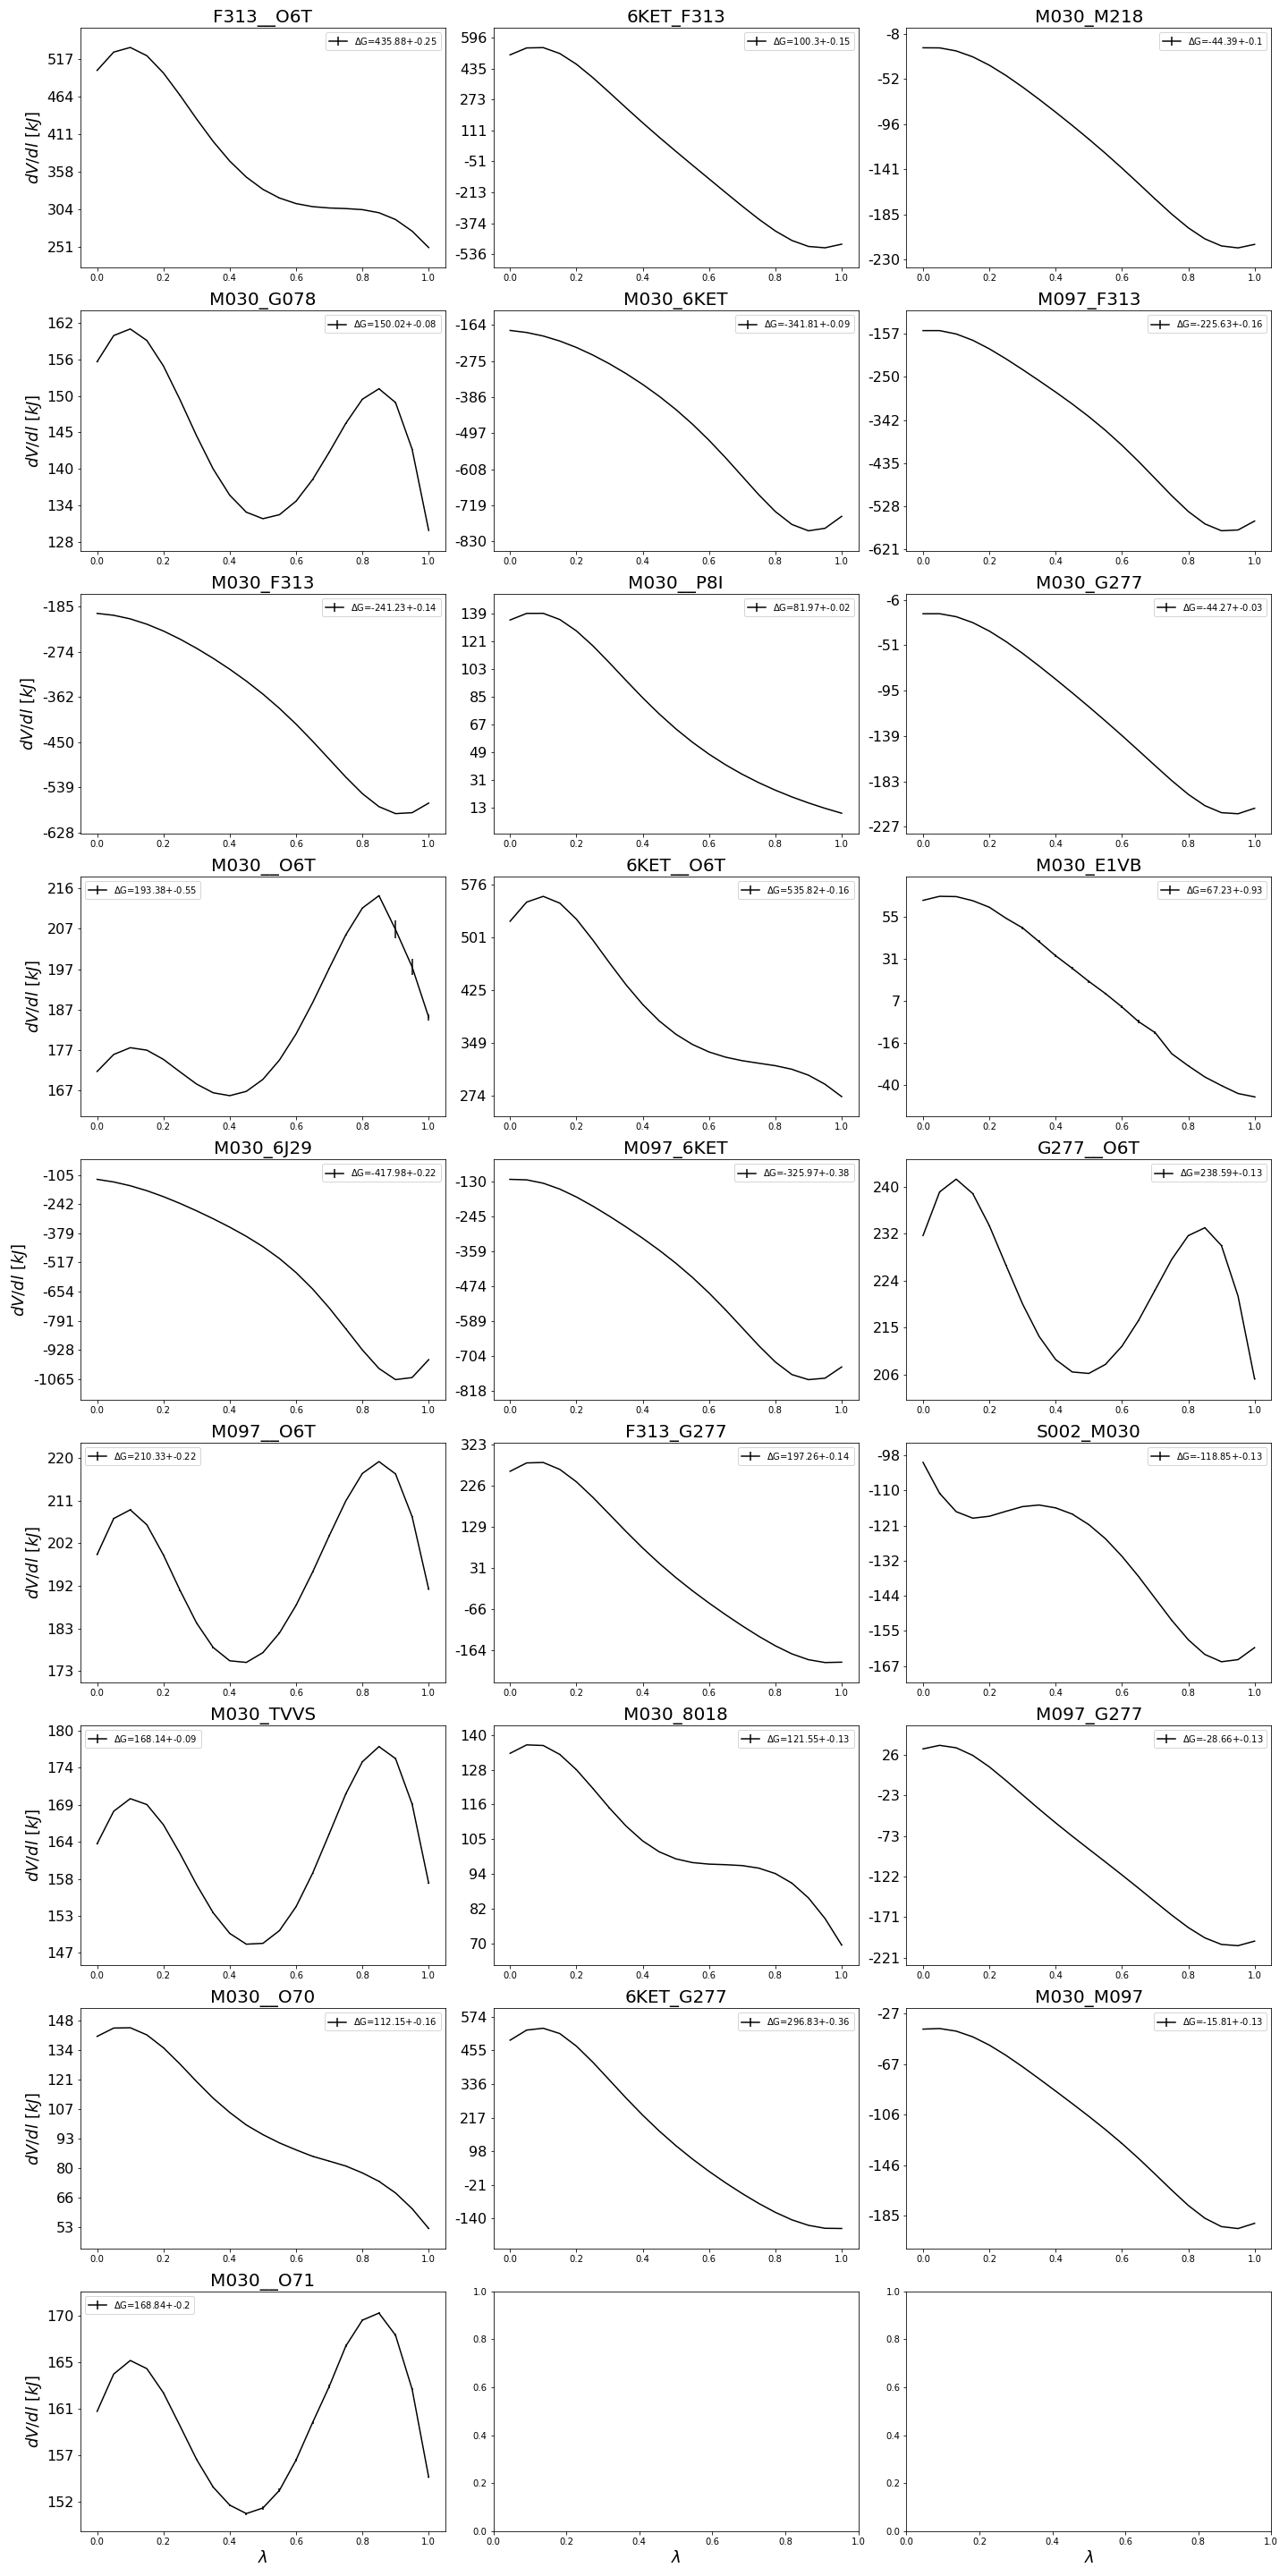
\includegraphics[width=0.65\textwidth]{fig/SI/dG_convergence/TI_vacuum_lambda_curves.png}
    \caption{Pairwise TI-Vacuum $\lambda$-curves}
    \label{SIfig:TI_vacuum_curve}
    \end{figure}

\begin{figure}
    \centering
    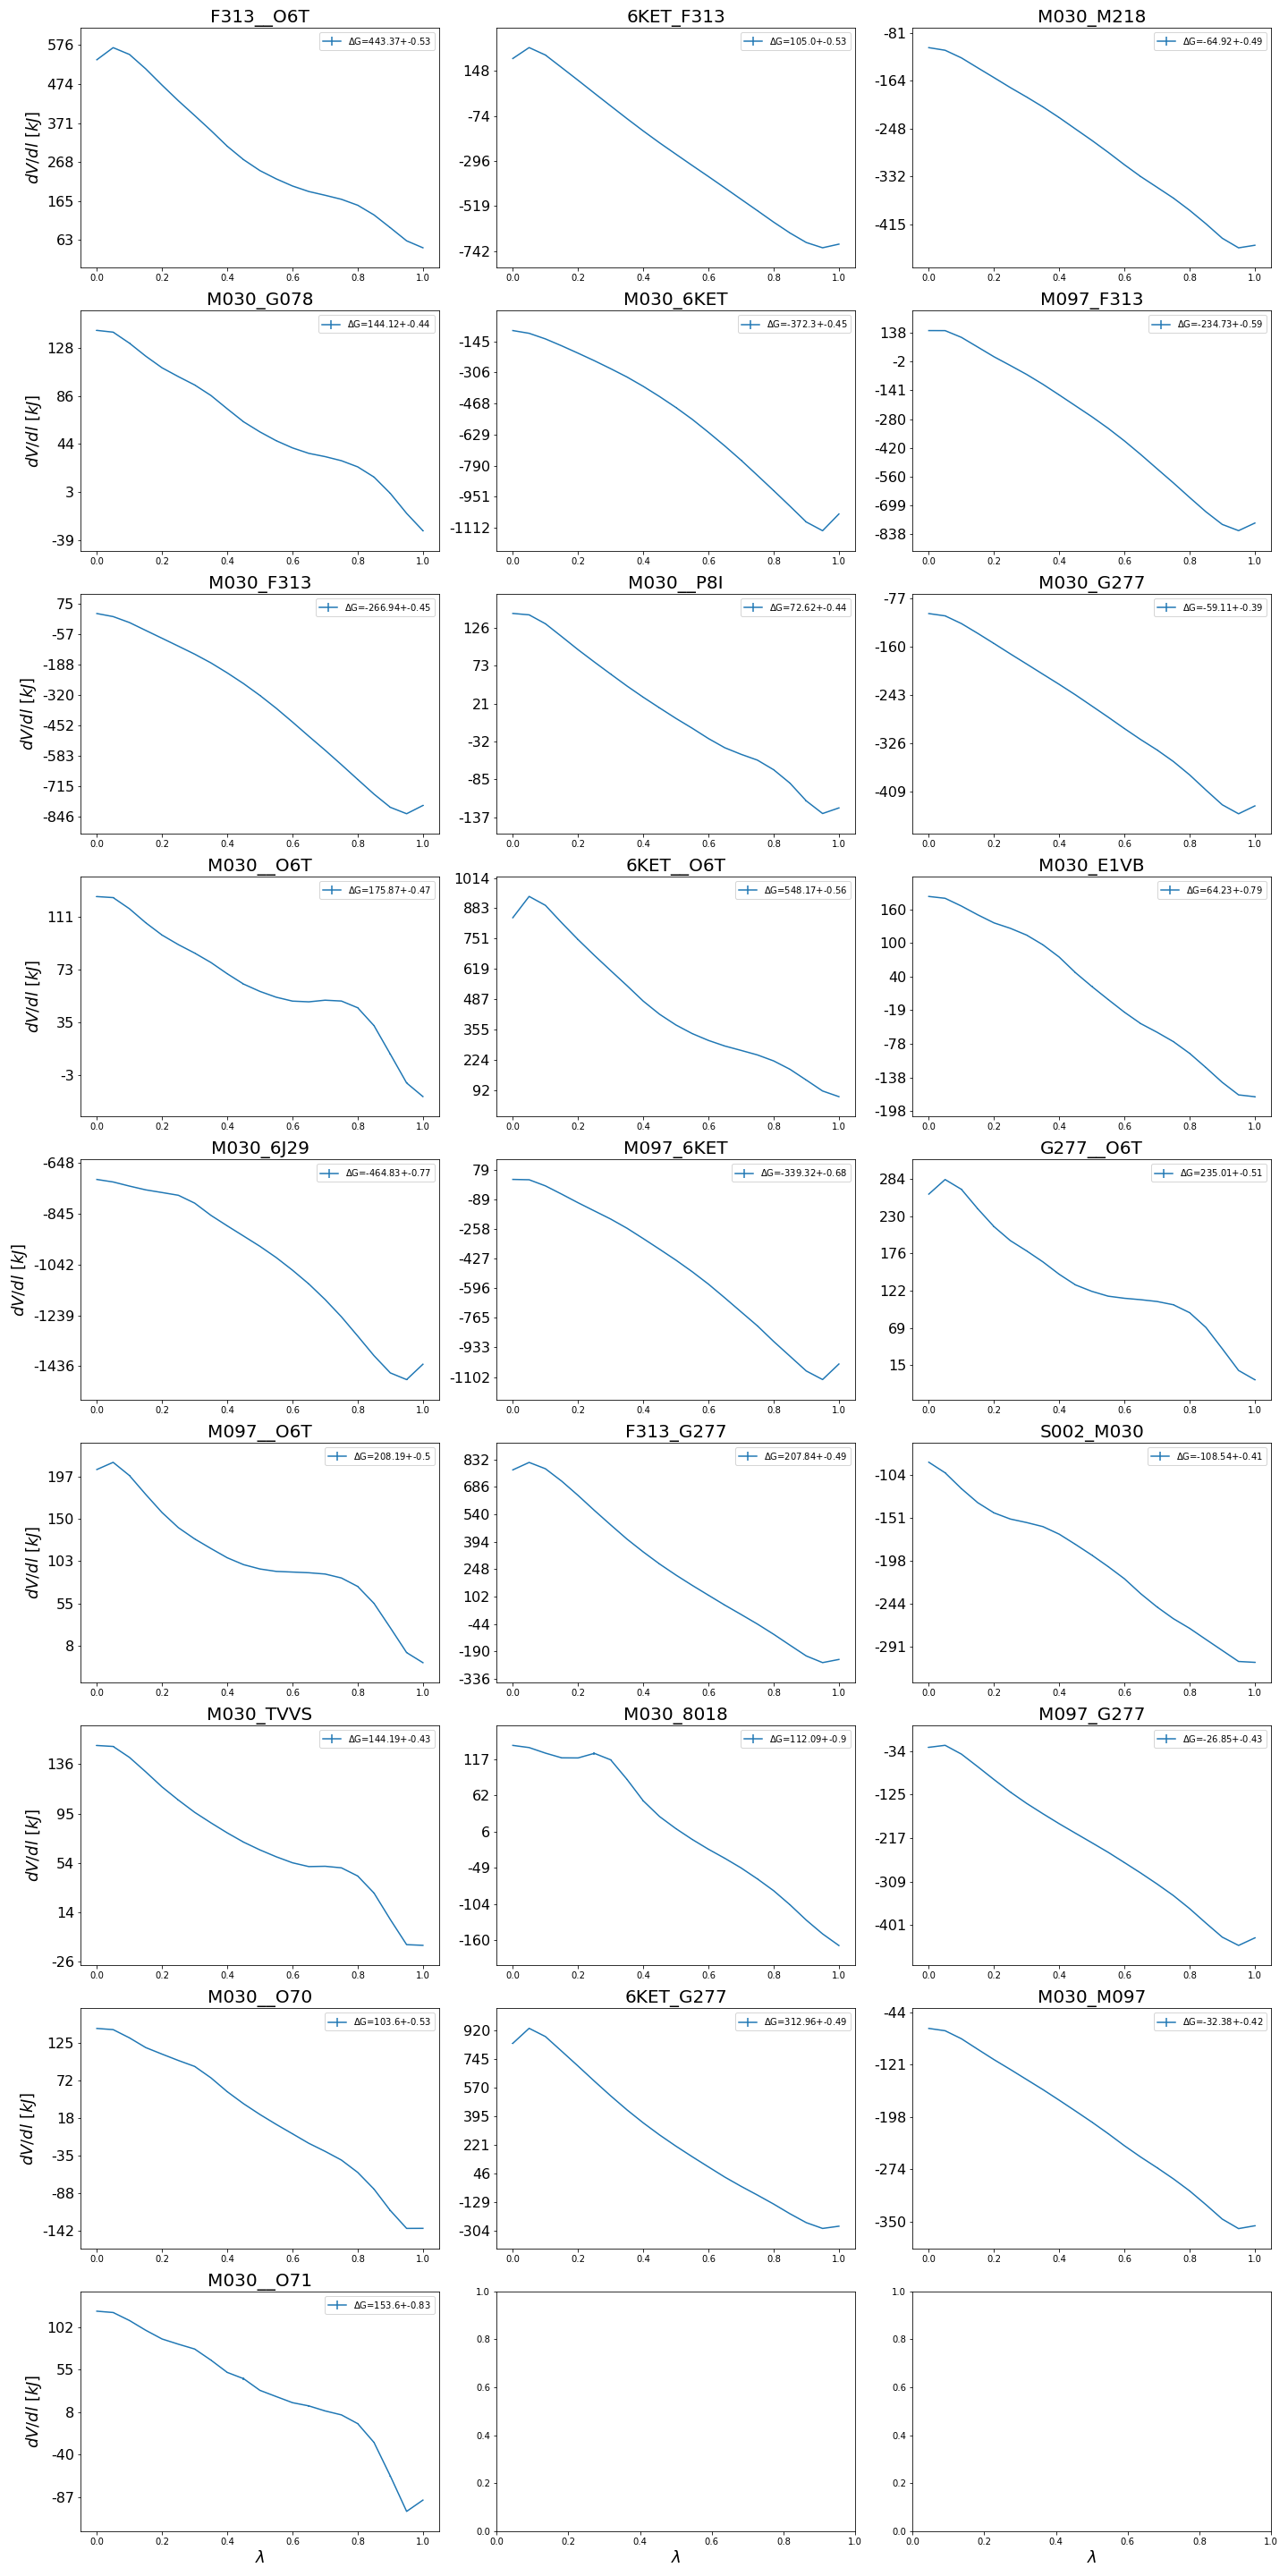
\includegraphics[width=0.65\textwidth]{fig/SI/dG_convergence/TI_water_lambda_curves.png}
    \caption{Pairwise TI-Water $\lambda$-curves}
    \label{SIfig:TI_water_curve}
\end{figure}

\begin{figure}
    \centering
    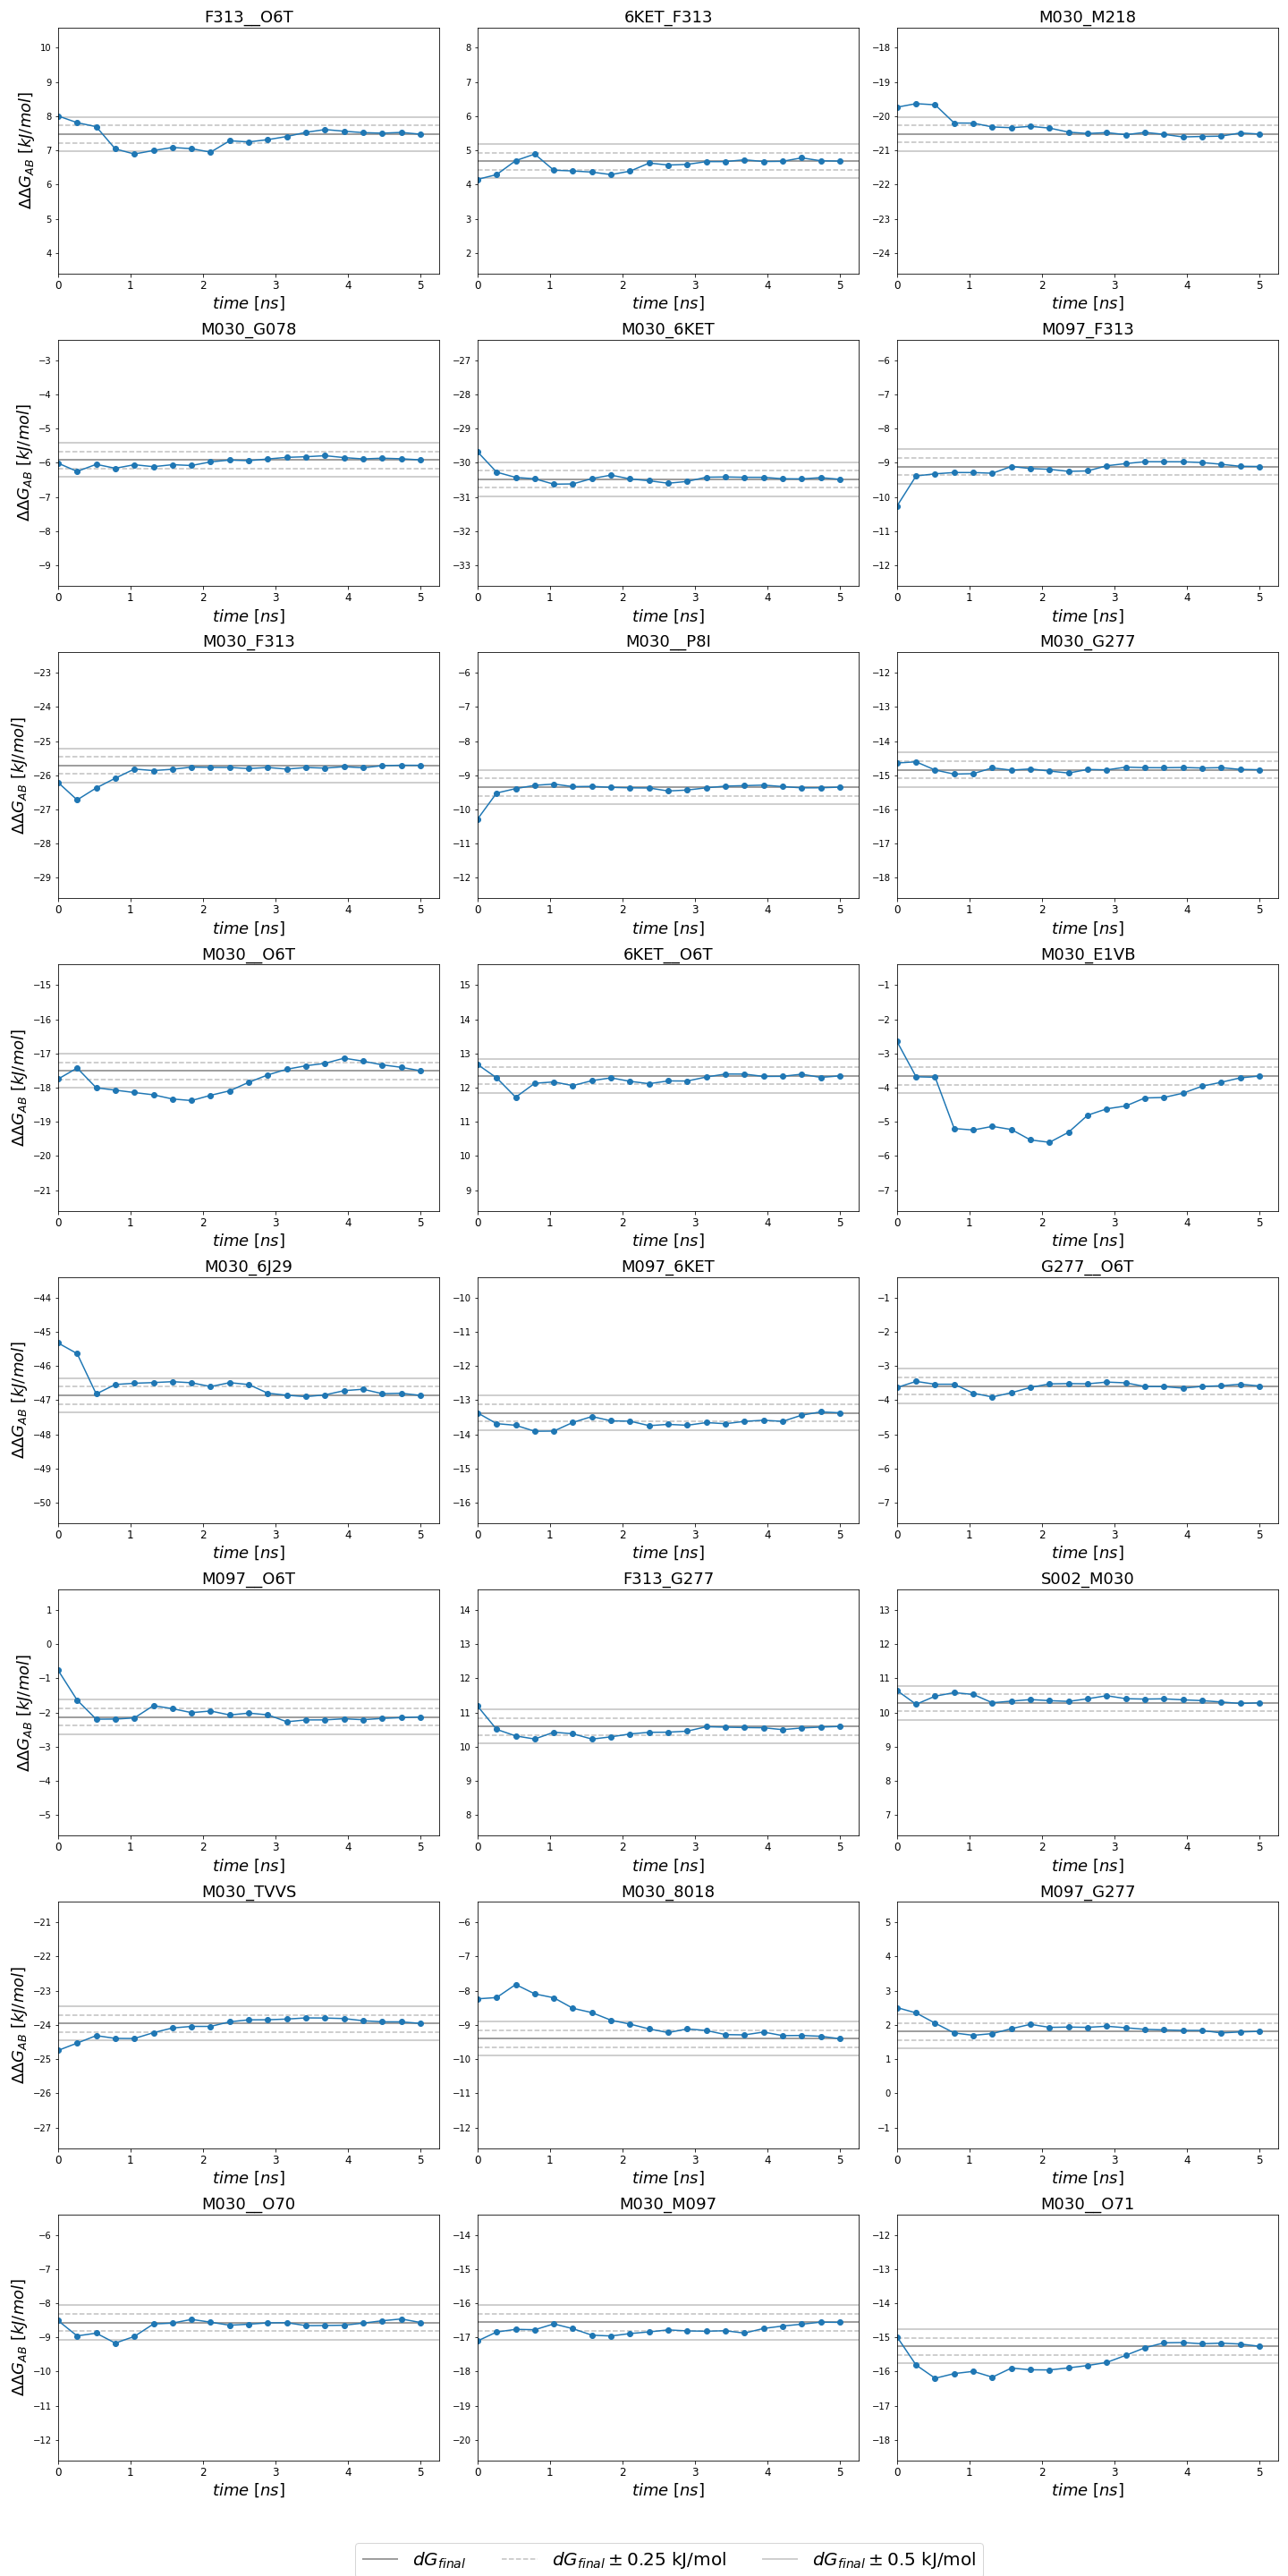
\includegraphics[width=0.65\textwidth]{fig/SI/dG_convergence/ddG_TI_convergence.png}
    \caption{time convergence of the pairwise TI free energy difference calculation of star-map Graph approach for ddG. (see Figure \ref{SIfig: Pairwise_TI_M030_Graph})}
    \label{fig: SI_figure df_convergence_TI}
\end{figure}
